\documentclass[fontsize=10pt, twoside=no]{scrartcl} % KOMA class

% other packages %
%\usepackage{graphicx}
\usepackage{titlesec}
%\usepackage{url}
\usepackage{fancybox}

% lang : french %
\usepackage[utf8]{inputenc}
\usepackage{xspace}
\usepackage[francais]{minitoc}
\usepackage{algorithm}
\usepackage{algorithmic}
\usepackage{graphicx}
\usepackage[T1]{fontenc}
\usepackage[english,frenchb]{babel}
%\usepackage[unicode,hidelinks]{hyperref}

% mise en page %
\pagestyle{empty}
\KOMAoptions{parskip=false}
\KOMAoptions{paper=a4,DIV=22}

\addto\captionsfrench{\def\partname{}}
\renewcommand{\thepart}{}
%%%%%%%%%%%%%%

\begin{document}

\title{MLEA : SVM(Support Vector Machine)}
\author{Thibault \textsc{Lapassade} - Florian \textsc{Thomassin}}
\date{}
\maketitle
\vspace*{-3cm}

\part{}

Le but de ce rapport est de présenter les résultats de notre étude des kernel de différents SVM dans le but de déterminer le plus efficace de ces kernels. Pour cela, on distinguera deux parties :

\begin{description}
\item[Les différents kernels] qui permettra de présenter les différents types de kernel choisit et le choix des paramètres pour chacun. ;
\item[Le benchmark] qui permettra de présenter grâce à des graphiques les résultats de chacune de nos expérimentations sur les kernels précédemment choisis.
\end{description}

Notre système de test est réalisé à l'aide de Matlab. Le format d'entrée des données d'acquisition est fixé et n'est pas le sujet d'étude de ce compte-rendu. On s'attardera plutôt à détailler l'analyse des kernels et du choix des paramètres de ceux-ci de manière à avoir la meilleur classification.

\part{Choix des kernels et des paramètres}

Il nous a fallut tout d'abord choisir une valeur de c correcte pour faire nos tests. Nous avons décidé de lancer nos tests sur différentes valeurs de c puisque nous nous sommes aperçus que cette valeur était souvent corrélés avec le taux d'erreurs de classification de plusieurs des kernels que nous avions choisit.\\

Une fois le choix de la valeur de c terminé, nous avons tout d'abord essayé le kernel linéaire qui est le kernel de base puisqu'il s'agit d'un simple produit scalaire. Nous nous sommes aperçus que les performances de ce kernel se rapprochait dans la pluspart des cas d'une classification aléatoire puisque le taux d'erreur lors de l'utilisation de ce kernel était d'environ 50{\%}.

Une fois ce premier kernel testé, nous avons décidé de tester le kernel polynomial. Pour faire ces tests, il nous a fallut décider de l'ordre du kernel polynomial que nous allions utilisés pour faire nos tests. Nous avons donc dans un premier temps utilisé un kernel polynomial d'ordre 2 puisque c'est le kernel se situant, pour ainsi dire, au dessus de kernel linéaire puisque le kernel polynomial d'ordre 1 peut s'apparenter à un kernel linéaire. Nous avons ensuite testé un kernel polynomial d'ordre plus haut puisque nous avons choisit d'utiliser un kernel polynomial d'ordre 4. Nous nous sommes aperçu que malgré ce changement d'ordre, nous avions toujours des taux d'erreurs assez proches de ceux avec un kernel polynomial d'ordre 2 et nous avons donc décidé de passer à un autre type de kernel.\\

\`A compléter

\part{Benchmark des kernels choisis}

\fbox{\begin{minipage}{0.9\textwidth}
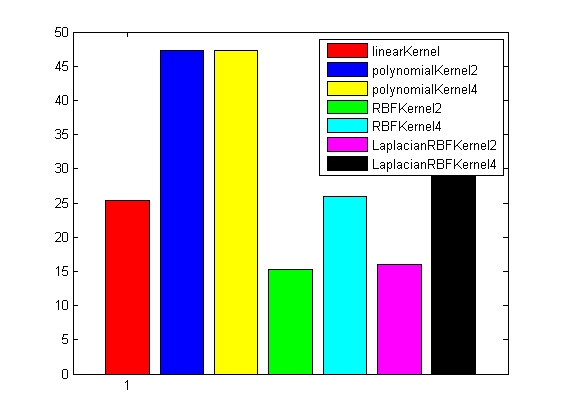
\includegraphics[scale=0.5]{image/c1.png}\\
\begin{center}
\textsc{c = 1}\\
\end{center}
\end{minipage}}\\


\fbox{\begin{minipage}{0.9\textwidth}
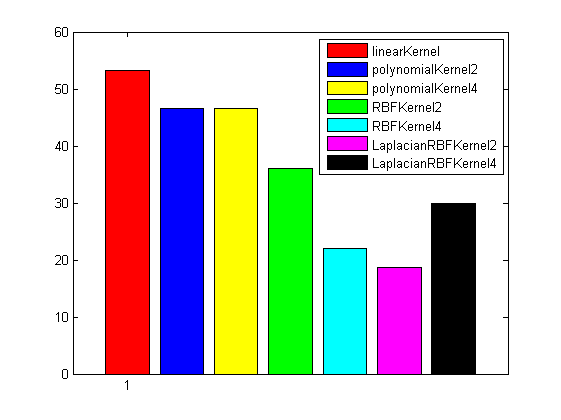
\includegraphics[scale=0.5]{image/c10.png}\\
\begin{center}
\textsc{c = 10}\\
\end{center}
\end{minipage}}\\


\fbox{\begin{minipage}{0.9\textwidth}
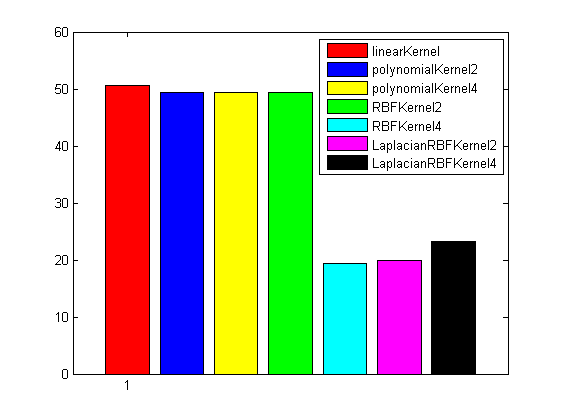
\includegraphics[scale=0.5]{image/c100.png}\\
\begin{center}
\textsc{c = 100}\\
\end{center}
\end{minipage}}\\


\fbox{\begin{minipage}{0.9\textwidth}
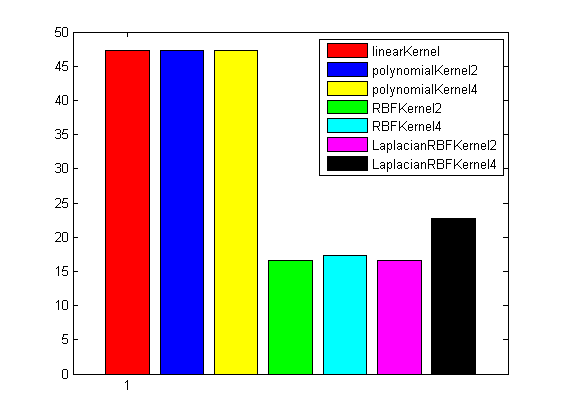
\includegraphics[scale=0.5]{image/c1000.png}\\
\begin{center}
\textsc{c = 1000}\\
\end{center}
\end{minipage}}\\


\fbox{\begin{minipage}{0.9\textwidth}
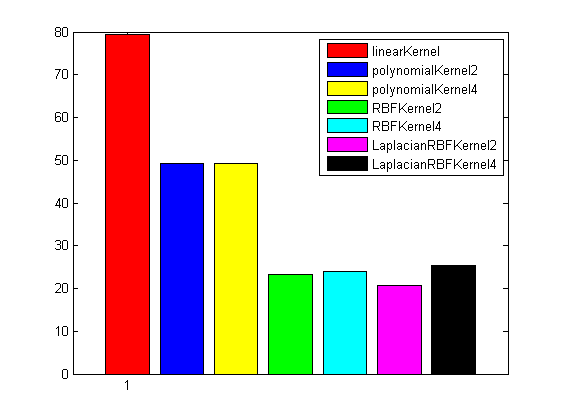
\includegraphics[scale=0.5]{image/c10000.png}\\
\begin{center}
\textsc{c = 10000}\\
\end{center}
\end{minipage}}\\

\part{Conclusion}

\`A partir des images des benchmarks précédents ainsi que grâce aux différents tests que nous avons pu effectué sur les différents kernels, on s'aperçoit que le kernel LaplacianRBF avec comme paramètre gamma=2 semble être le kernel le plus a même de bien classifier les données dont nous disposons pour le test. Néanmoins, il ne faut pas oublier que nos benchmark ont été uniquement effectué sur le set de data iris et pas sur le set de data opdigit pour cause de problème lors de l'apprentissage sur ce set et que nos résultats sont peut être biaisés par ce manque de données de test et ne reflètent donc peut être pas la réalité.


\end{document}
